\documentclass[10pt,twocolumn]{article}

% ── Packages ──────────────────────────────────────────────────
\usepackage[margin=1.8cm, top=2.2cm, bottom=2.2cm]{geometry}
\usepackage{amsmath, amssymb}
\usepackage{graphicx}
\usepackage{booktabs}
\usepackage{array}
\usepackage{tabularx}
\usepackage{xcolor}
\usepackage{hyperref}
\usepackage{natbib}
\usepackage{caption}
\usepackage{subcaption}
\usepackage{float}
\setlength{\textfloatsep}{8pt plus 2pt minus 2pt}
\setlength{\floatsep}{6pt plus 2pt minus 2pt}
\setlength{\intextsep}{6pt plus 2pt minus 2pt}
\usepackage{microtype}
\usepackage{authblk}
\usepackage{abstract}
\usepackage{titlesec}
\usepackage{parskip}
\usepackage{fancyhdr}
\usepackage{fontenc}
\usepackage{inputenc}
\usepackage{lmodern}
\usepackage{multicol}
\usepackage{mdframed}
\usepackage{colortbl}
\usepackage{threeparttable}

% ── Colors ────────────────────────────────────────────────────
\definecolor{navy}{HTML}{0D1B2A}
\definecolor{teal}{HTML}{1A7A8A}
\definecolor{coral}{HTML}{E05A3A}
\definecolor{lgrey}{HTML}{E8EDF2}
\definecolor{textgrey}{HTML}{4A5568}

% ── Section formatting ────────────────────────────────────────
\titleformat{\section}
  {\color{navy}\normalfont\large\bfseries}
  {\thesection}{1em}{}[\color{navy}\titlerule]

\titleformat{\subsection}
  {\color{teal}\normalfont\normalsize\bfseries}
  {\thesubsection}{1em}{}

\titlespacing{\section}{0pt}{10pt}{4pt}
\titlespacing{\subsection}{0pt}{6pt}{2pt}

% ── Header / Footer ───────────────────────────────────────────
\pagestyle{fancy}
\fancyhf{}
\renewcommand{\headrulewidth}{1.5pt}
\renewcommand{\headrule}{\hbox to\headwidth{\color{navy}\leaders\hrule height \headrulewidth\hfill}}
\fancyhead[L]{\small\color{navy}\textbf{AuDHD Network Study}}
\fancyhead[R]{\small\color{navy}\thepage}
\fancyfoot[C]{\footnotesize\color{textgrey}Differential Co-Expression Network Architecture --- AuDHD Molecular Targets}

% ── Caption formatting ────────────────────────────────────────
\captionsetup{font=small, labelfont=bf, textfont=it,
              format=plain, justification=centering}

% ── Abstract formatting ───────────────────────────────────────
\renewcommand{\abstractnamefont}{\normalfont\bfseries\color{white}}
\renewcommand{\abstracttextfont}{\normalfont\small}

% ── Hyperlink colors ──────────────────────────────────────────
\hypersetup{
    colorlinks=true,
    linkcolor=teal,
    citecolor=teal,
    urlcolor=teal
}

% ═════════════════════════════════════════════════════════════
\begin{document}

% ── TITLE (full width) ────────────────────────────────────────
\twocolumn[{%
\begin{@twocolumnfalse}

\begin{center}
  {\LARGE\bfseries\color{navy}
    Differential Co-Expression Network Architecture as a Framework\\
    for Defining AuDHD-Associated Molecular Targets
  \par}
  \vspace{0.5em}

  {\large [Your Name]$^{1}$}\\[0.3em]
  {\small\color{textgrey}
    $^{1}$Independent Bioinformatics Research Project, Supervised Research\\
    Correspondence: \texttt{[your email]} $\bullet$
    \url{github.com/vedika13-code/AuDHD-Network}
  }

  \vspace{0.8em}
  \noindent\color{navy}\rule{\linewidth}{1.5pt}
  \vspace{0.5em}
\end{center}

% ── ABSTRACT BOX ──────────────────────────────────────────────
\begin{mdframed}[
  backgroundcolor=lgrey,
  linecolor=navy,
  linewidth=1pt,
  innertopmargin=8pt,
  innerbottommargin=8pt,
  innerleftmargin=10pt,
  innerrightmargin=10pt
]
{\color{navy}\bfseries Abstract}\\[4pt]
\small
\textbf{Background:} Autism spectrum disorder (ASD) and attention-deficit/hyperactivity
disorder (ADHD) co-occur in up to 70\% of cases, yet differential gene expression studies
find minimal direct gene-level overlap. We propose ASD-ADHD overlap exists at the level of
co-expression network architecture rather than individual gene changes.

\medskip
\textbf{Methods:} We constructed a weighted gene co-expression network (WGCNA) from 238
ASD and typically developing control whole blood samples (GSE111175 + GSE42133). Module-trait
association identified the primary ASD module. Hub genes were validated against STRING v11.5
protein-protein interaction (PPI) data using degree centrality (Wilcoxon test). Cross-disorder
validation tested ME11 dysregulation in ADHD (GSE159104, n=76). Reactome pathway enrichment
characterized module biology.

\medskip
\textbf{Results:} WGCNA identified 33 modules; ME11 was the primary ASD-associated module
($r=-0.26$, FDR$=0.0008$, 298 genes). Five hub genes were identified: TMSB4X, RAP1B, HSPCAL3,
C1D, ZCCHC10. Hub genes did not show elevated PPI centrality (Wilcoxon $p=0.37$). ME11 was
not dysregulated in ADHD ($p=0.825$). Reactome enrichment identified four FDR-significant
spliceosomal pathways (mRNA Splicing FDR$=0.007$).

\medskip
\textbf{Conclusions:} ME11 is an ASD-specific spliceosomal co-expression module reflecting
transcriptional co-regulation. The WGCNA-PPI framework distinguishes disorder-specific from
shared molecular networks, providing a reproducible foundation for computationally defining
AuDHD biology.

\medskip
\textit{\textbf{Keywords:} AuDHD $\bullet$ WGCNA $\bullet$ co-expression networks $\bullet$
autism $\bullet$ ADHD $\bullet$ PPI $\bullet$ spliceosome $\bullet$ mRNA splicing $\bullet$
blood transcriptomics}
\end{mdframed}

\vspace{1em}
\noindent\color{lgrey}\rule{\linewidth}{0.5pt}
\vspace{0.5em}

\end{@twocolumnfalse}
}]

% ═══════════════════════════════════════════════════════════════
% TWO-COLUMN CONTENT
% ═══════════════════════════════════════════════════════════════

\section{Introduction}

ASD and ADHD are among the most prevalent neurodevelopmental conditions worldwide.
Epidemiological studies estimate that 50--70\% of individuals with ASD also meet diagnostic
criteria for ADHD, a co-occurrence increasingly recognized as ``AuDHD'' \citep{vanderbilt2024,
apa2024}. Despite this striking clinical overlap, the molecular basis of ASD-ADHD
comorbidity remains poorly understood.

Gene-level studies find surprisingly limited overlap between ASD and ADHD \citep{mallard2024}.
We propose this paradox arises because shared biology is encoded in gene regulatory network
organization rather than individual genes --- a level of biological complexity requiring
systems-level analytical frameworks.

Weighted Gene Co-expression Network Analysis (WGCNA) identifies co-expressed gene modules
reflecting shared regulatory inputs \citep{langfelder2008}. Applied to ASD postmortem brain,
WGCNA demonstrated convergent transcriptional and splicing dysregulation across genetically
heterogeneous cases \citep{voineagu2011}. For ADHD, WGCNA on peripheral blood mononuclear
cells identified co-expression modules associated with ADHD status \citep{thapar2022}.
However, no study has jointly interrogated ASD and ADHD transcriptomes to define shared
versus disorder-specific network architecture.

Complementing co-expression analysis, protein-protein interaction (PPI) network analysis
maps physical interactions between protein products. Convergence of co-expression hub gene
identity with PPI centrality provides strong evidence for druggable protein complexes
\citep{nangraj2020}. This WGCNA-PPI integration has not previously been applied to
neurodevelopmental comorbidity.

Here we construct an ASD co-expression network (n$=238$), identify ME11 as the primary
ASD-associated module, validate hub genes against STRING PPI, cross-validate ME11 in ADHD
(n$=76$), and characterize biology through Reactome pathway enrichment. This provides the
first network-topological characterization of AuDHD-relevant molecular architecture.

% ═══════════════════════════════════════════════════════════════
\section{Methods}

\subsection{Dataset Selection}

ASD datasets: GSE111175 and GSE42133 (whole blood leukocytes, Illumina HumanHT-12 V4.0,
GPL10558; Pramparo/Courchesne lab, UC San Diego; toddlers aged 11--45 months). ADHD
dataset: GSE159104 (whole blood RNA-seq, Helicos HeliScope, GPL14761; twin-pair discordant
design). All datasets retrieved from NCBI GEO using GEOquery \citep{davis2007}.

\subsection{Preprocessing}

\textbf{ASD:} Datasets merged on 47,323 common probes (n$=245$). ComBat batch correction
\citep{johnson2007} applied and validated by PCA (Figure~\ref{fig:pca}). Rank-based
inverse normal transformation (RINT) was tested and rejected --- it destroyed inter-sample
correlation structure ($r\approx0$ post-RINT) required for WGCNA. Top 15,000 most variable
probes selected; seven outlier samples removed (Z$<-2.5$). Final matrix:
$15{,}000 \times 238$ samples (115 ASD, 123 TD).

\textbf{ADHD:} Protein-coding genes retained (24,477 $\rightarrow$ 11,964 after expression
filtering); technical replicates averaged per individual. Final matrix:
$11{,}964 \times 76$ samples (39 ADHD, 37 CTRL).

\subsection{WGCNA Network Construction}

WGCNA performed on ASD dataset \citep{langfelder2008}. ADHD dataset unsuitable due to
insufficient sample size (n$=76$; maximum scale-free R$^2=0.53$ across powers 1--20).
Signed network constructed with $\beta=12$ (R$^2=0.88$, $\bar{k}=30.9$). Modules identified
by hierarchical clustering (minimum size 30, merge cut height 0.25).

\subsection{Module-Trait Association \& Hub Genes}

Module eigengenes correlated with binary ASD diagnosis (Pearson $r$; Benjamini-Hochberg
FDR correction). Hub genes defined by joint criteria: $|\text{MM}|>0.8$ AND
$|\text{GS}|>0.2$, mapped to HGNC symbols via GPL10558 annotation.

\subsection{PPI Validation}

PPI data from STRING v11.5 \citep{szklarczyk2023} (combined score $\geq400$). Network
constructed using igraph. Degree and betweenness centrality computed. Centrality convergence
tested: one-sided Wilcoxon rank-sum test, hub genes vs background ME11 genes.

\subsection{ADHD Validation}

Differential expression via limma \citep{ritchie2015}. Module score $=$ mean z-score
across 79 ME11 genes identified in ADHD matrix (after UCSC-to-symbol mapping). Group
comparison: two-sample $t$-test. ME11 enrichment among ADHD DE genes: Fisher's exact test.

\subsection{Pathway Enrichment}

GO enrichment: clusterProfiler \citep{yu2012}, org.Hs.eg.db, BP/MF/CC ontologies.
Reactome enrichment: ReactomePA \citep{yu2016}. Both with BH FDR correction
(significance threshold FDR$<0.05$).

% ═══════════════════════════════════════════════════════════════
\section{Results}

\subsection{Preprocessing \& Quality Control}

Strong batch effects between GSE111175 and GSE42133 confirmed by PCA (complete PC1
separation) and resolved by ComBat (Figure~\ref{fig:pca}). Seven ASD outliers removed.
Final cohorts: ASD 238 samples (115 ASD, 123 TD); ADHD 76 samples (39 ADHD, 37 CTRL).

\begin{figure}[!htbp]
  \centering
  \begin{subfigure}[b]{0.48\columnwidth}
    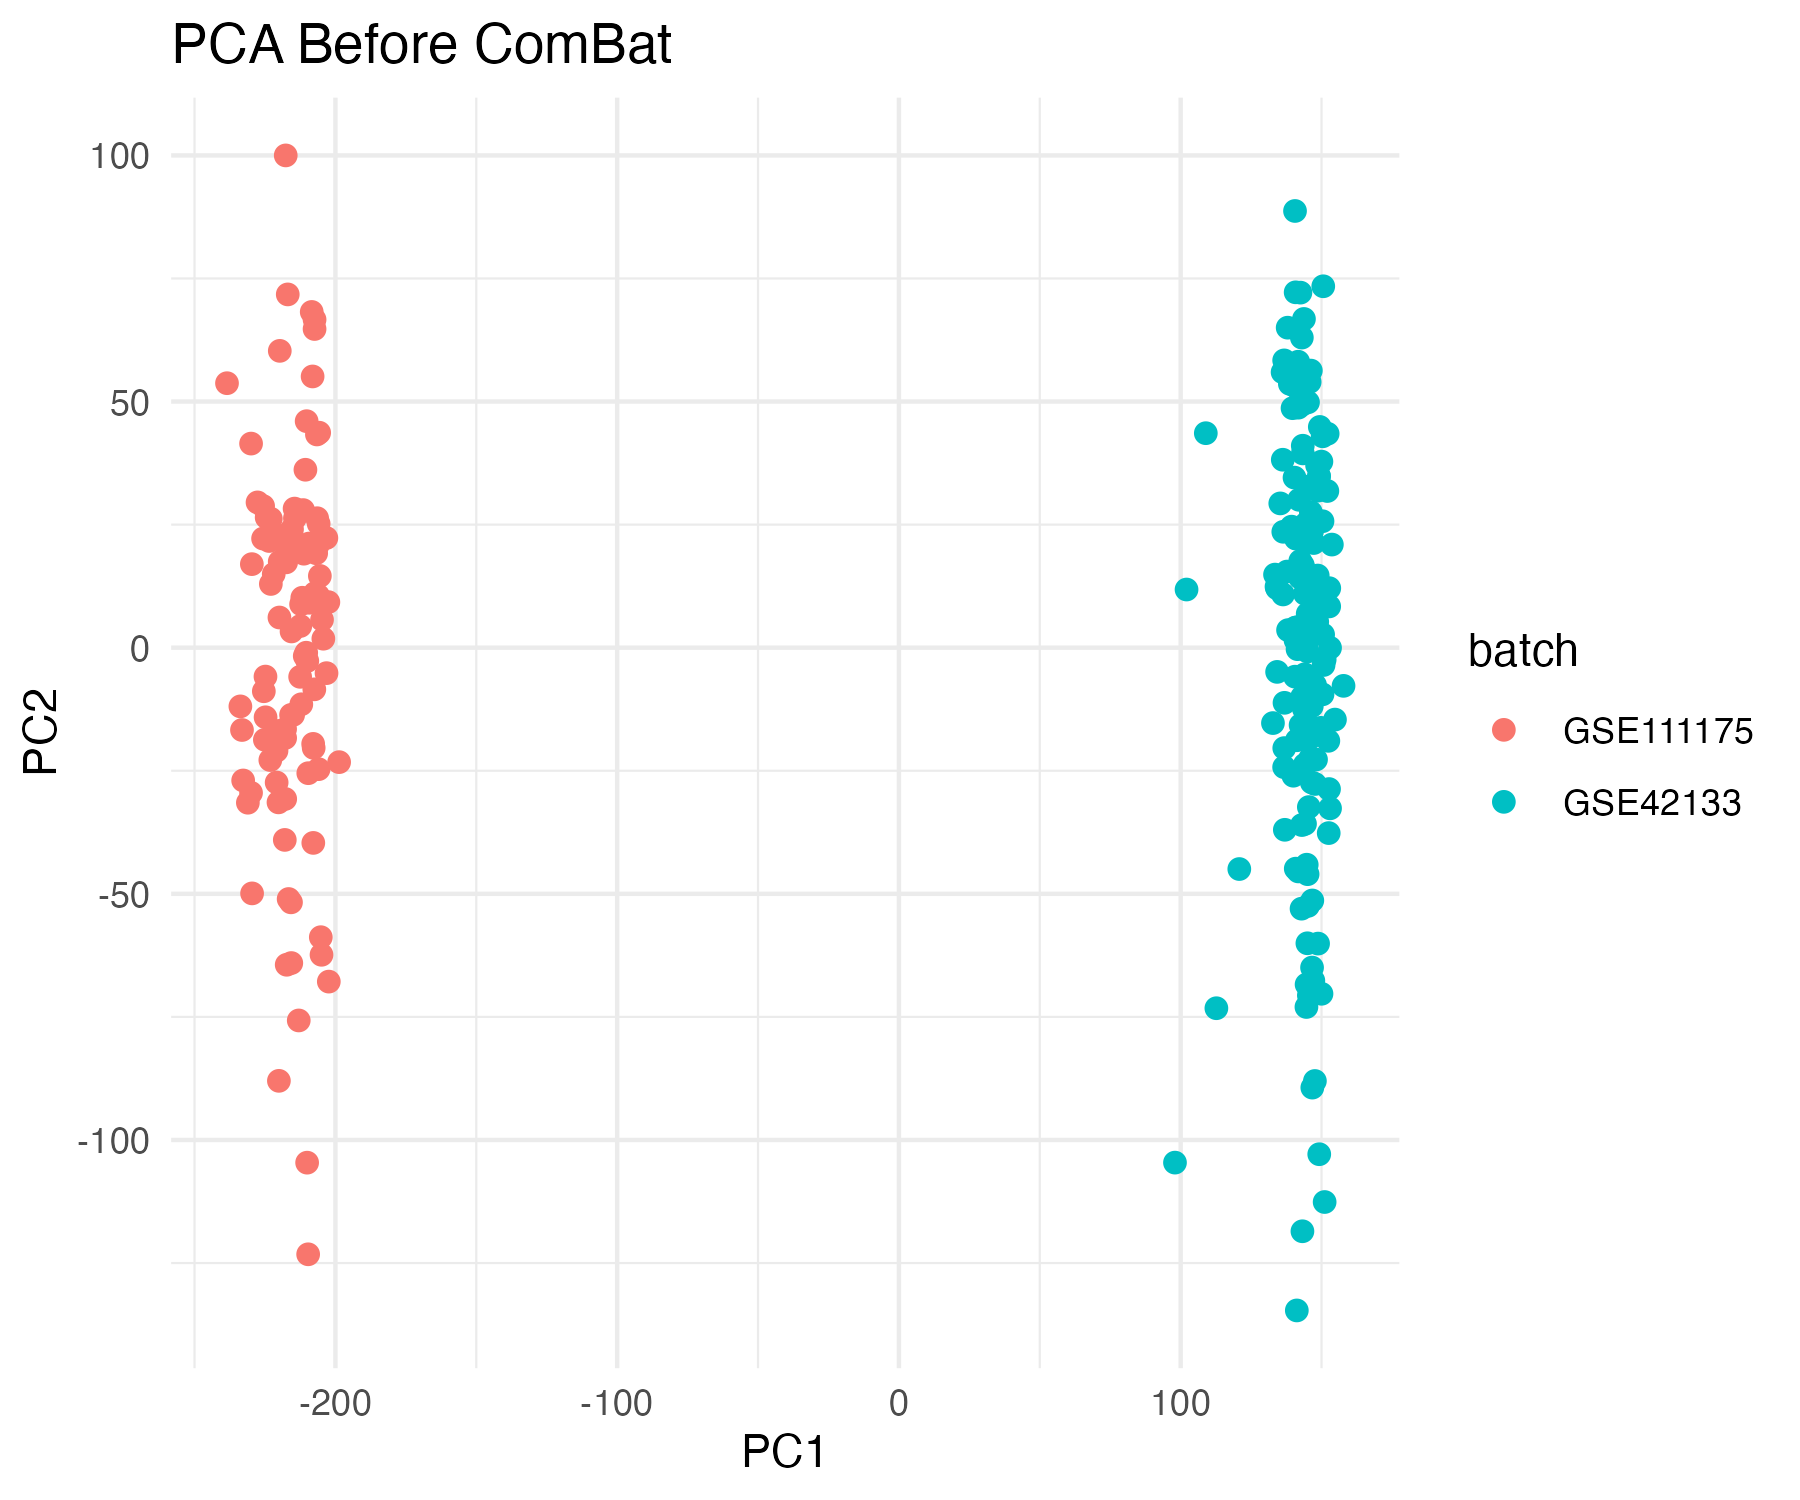
\includegraphics[width=\linewidth]{pca_asd_before_combat.png}
    \caption*{Before ComBat}
  \end{subfigure}
  \hfill
  \begin{subfigure}[b]{0.48\columnwidth}
    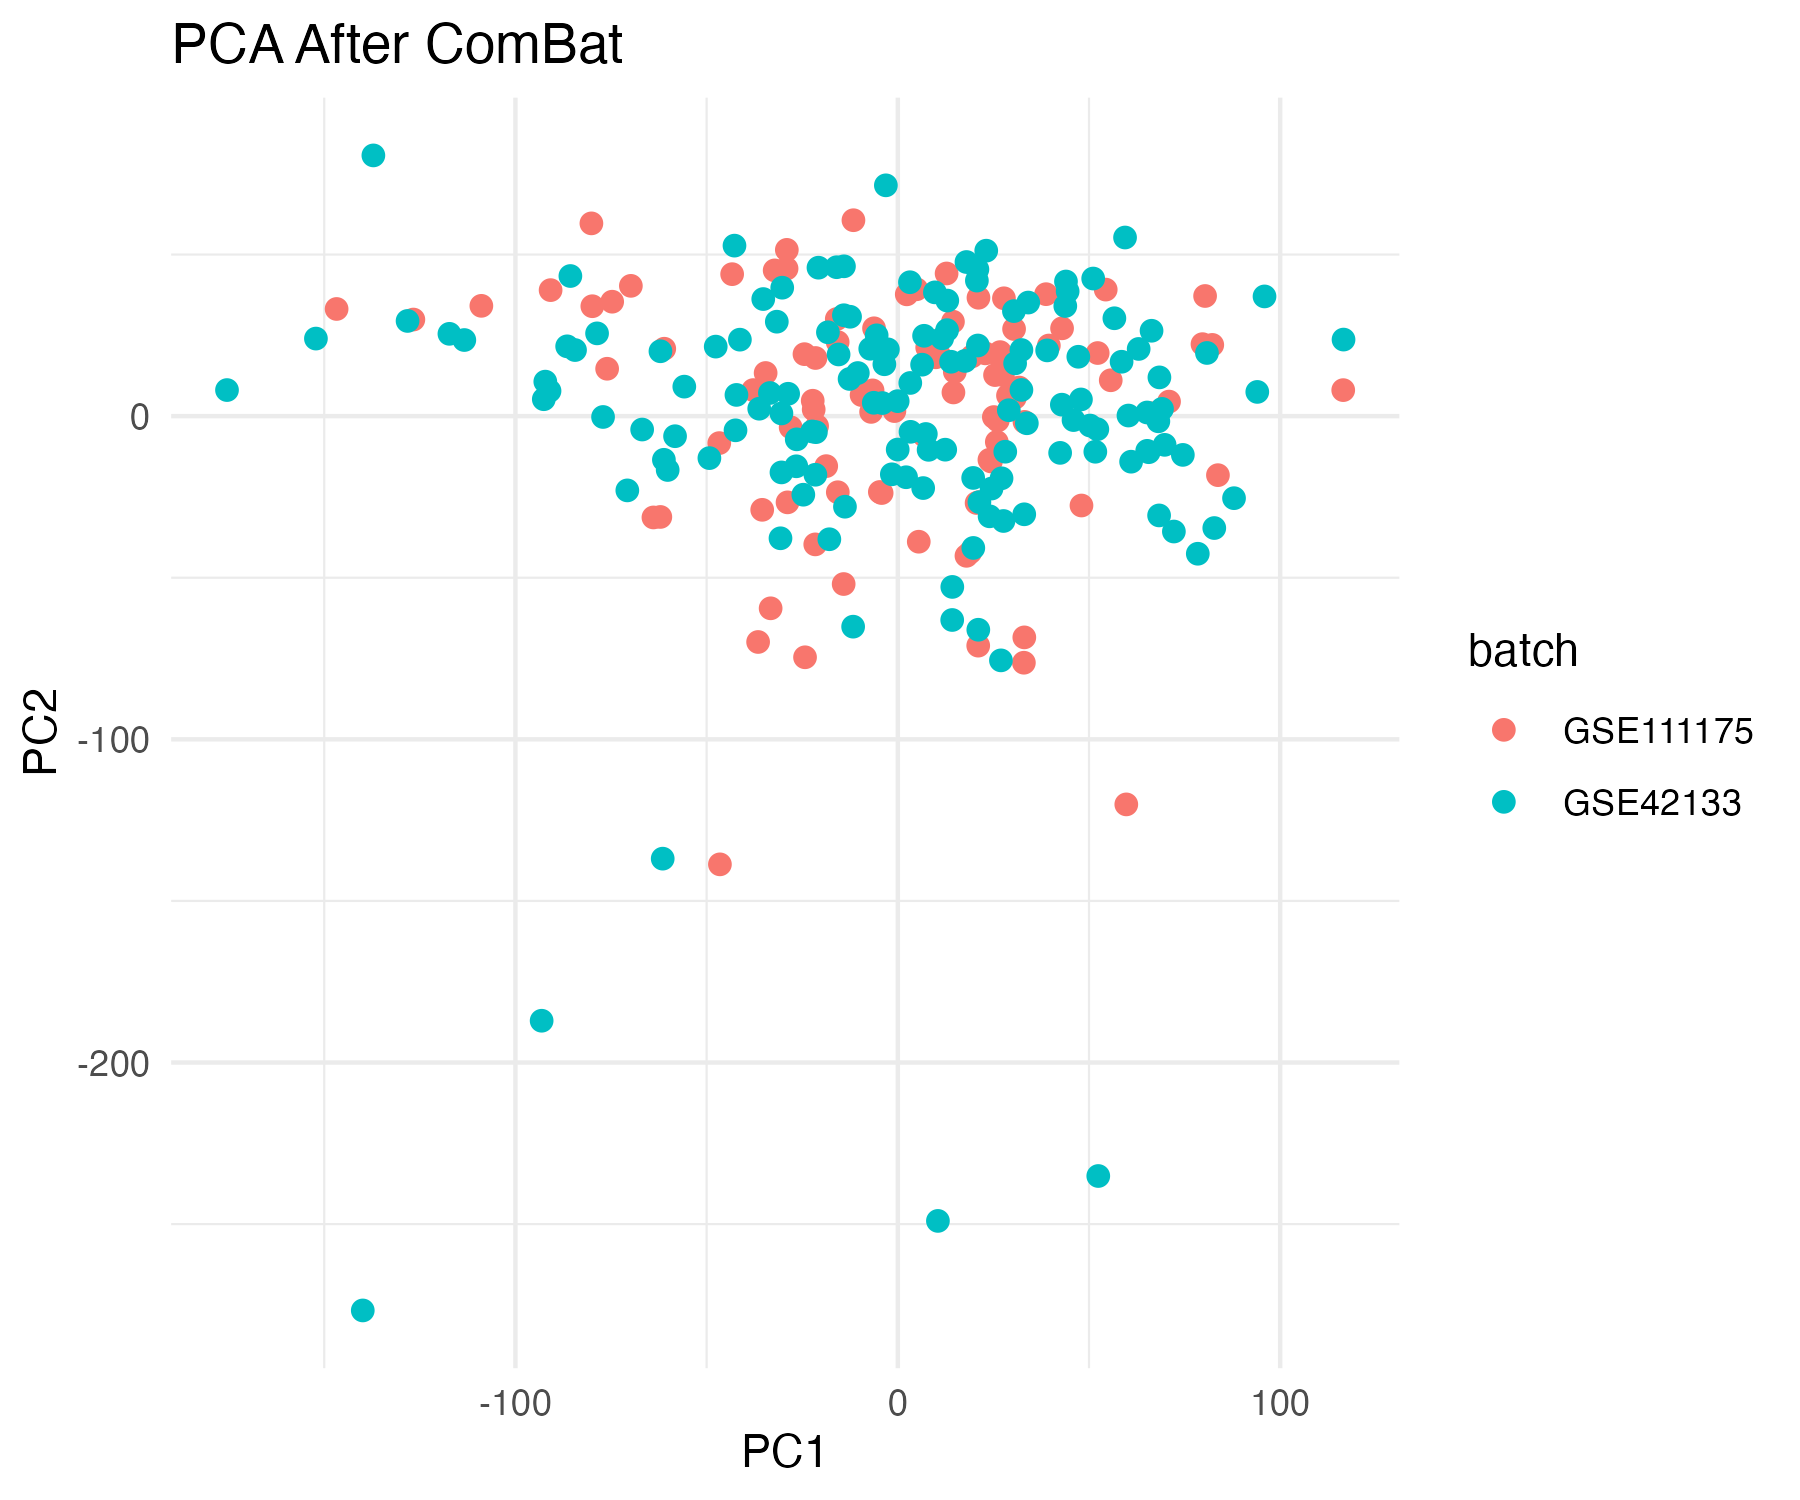
\includegraphics[width=\linewidth]{pca_asd_after_combat.png}
    \caption*{After ComBat}
  \end{subfigure}
  \caption{PCA of merged ASD data before and after ComBat batch correction. Complete PC1
  separation confirms strong batch effect; intermixing after correction validates the
  ComBat procedure.}
  \label{fig:pca}
\end{figure}

\subsection{WGCNA --- 33 Modules Detected}

WGCNA with $\beta=12$ (R$^2=0.88$) detected 33 co-expression modules
(Figure~\ref{fig:dendro}). Module sizes ranged from 33 to 1,660 genes; grey module
(22\% unassigned) excluded from all analyses. WGCNA not feasible on ADHD dataset
(maximum R$^2=0.53$, n$=76$ insufficient).

\begin{figure}[!htbp]
  \centering
  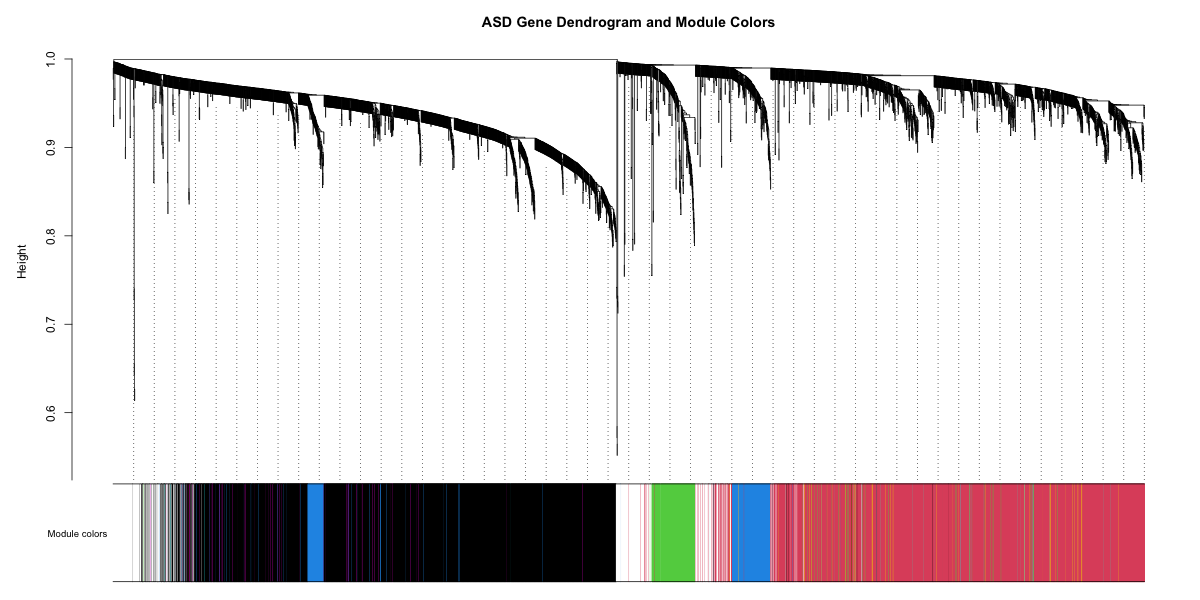
\includegraphics[width=\columnwidth]{ASD_dendrogram_final.png}
  \caption{ASD gene co-expression network dendrogram. 33 modules detected; color bar shows
  module assignments. Grey $=$ unassigned (22\%).}
  \label{fig:dendro}
\end{figure}

\subsection{ME11 --- Primary ASD-Associated Module}

ME11 was significantly negatively correlated with ASD diagnosis ($r=-0.26$, FDR$=0.0008$,
298 genes; Figure~\ref{fig:heatmap}), indicating lower eigengene expression in ASD
relative to TD controls. No other module survived FDR$<0.05$.

\begin{figure}[!htbp]
  \centering
  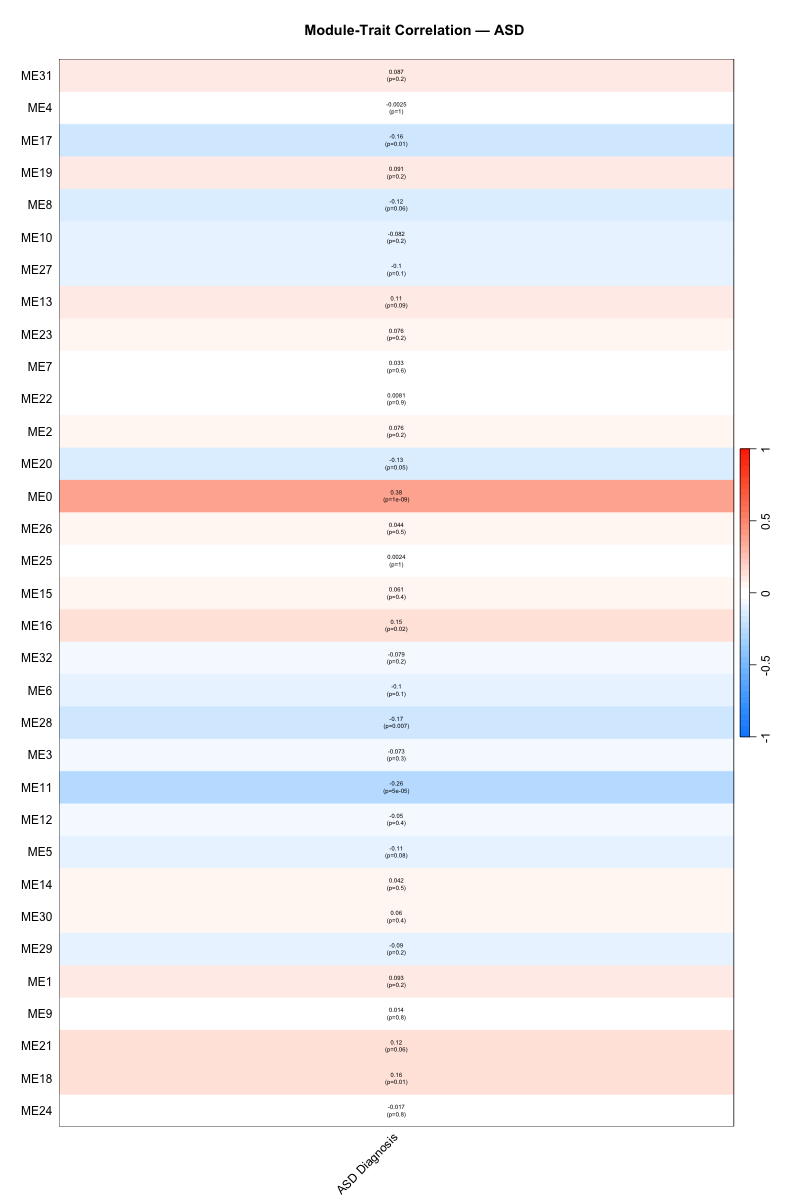
\includegraphics[width=\columnwidth]{ASD_module_trait_heatmap.png}
  \caption{Module-trait correlation heatmap. ME11 ($r=-0.26$, FDR$=0.0008$) is the
  primary ASD-associated module. ME0 excluded (grey module).}
  \label{fig:heatmap}
\end{figure}

\subsection{Hub Gene Identification}

Five characterized hub genes identified from ME11 ($|\text{MM}|>0.8$, $|\text{GS}|>0.2$):

\begin{table}[!htbp]
\centering
\caption{ME11 hub genes and biological functions.}
\label{tab:hubs}
\begin{tabular}{>{\bfseries}ll}
\toprule
\rowcolor{navy}\color{white}Gene & \color{white}Function \\
\midrule
TMSB4X  & Actin dynamics; neuroprotection \\
\rowcolor{lgrey}
RAP1B   & RAS GTPase; integrin signaling \\
HSPCAL3 & Heat shock; protein folding \\
\rowcolor{lgrey}
C1D     & Nuclear corepressor; DNA repair \\
ZCCHC10 & RNA-binding; splicing regulation \\
\bottomrule
\end{tabular}
\end{table}

\subsection{PPI Centrality --- Non-Convergence}

ME11 PPI network comprised 127 nodes and 195 edges (Figure~\ref{fig:ppi}). Hub gene
degree centrality ranged from the 19th (TMSB4X) to 67th percentile (RAP1B, C1D, ZCCHC10).
Wilcoxon test revealed no significant centrality difference between hub and background ME11
genes (W$=194$, $p=0.37$) --- ME11 reflects transcriptional co-regulation, not a
protein complex.

\begin{figure}[!htbp]
  \centering
  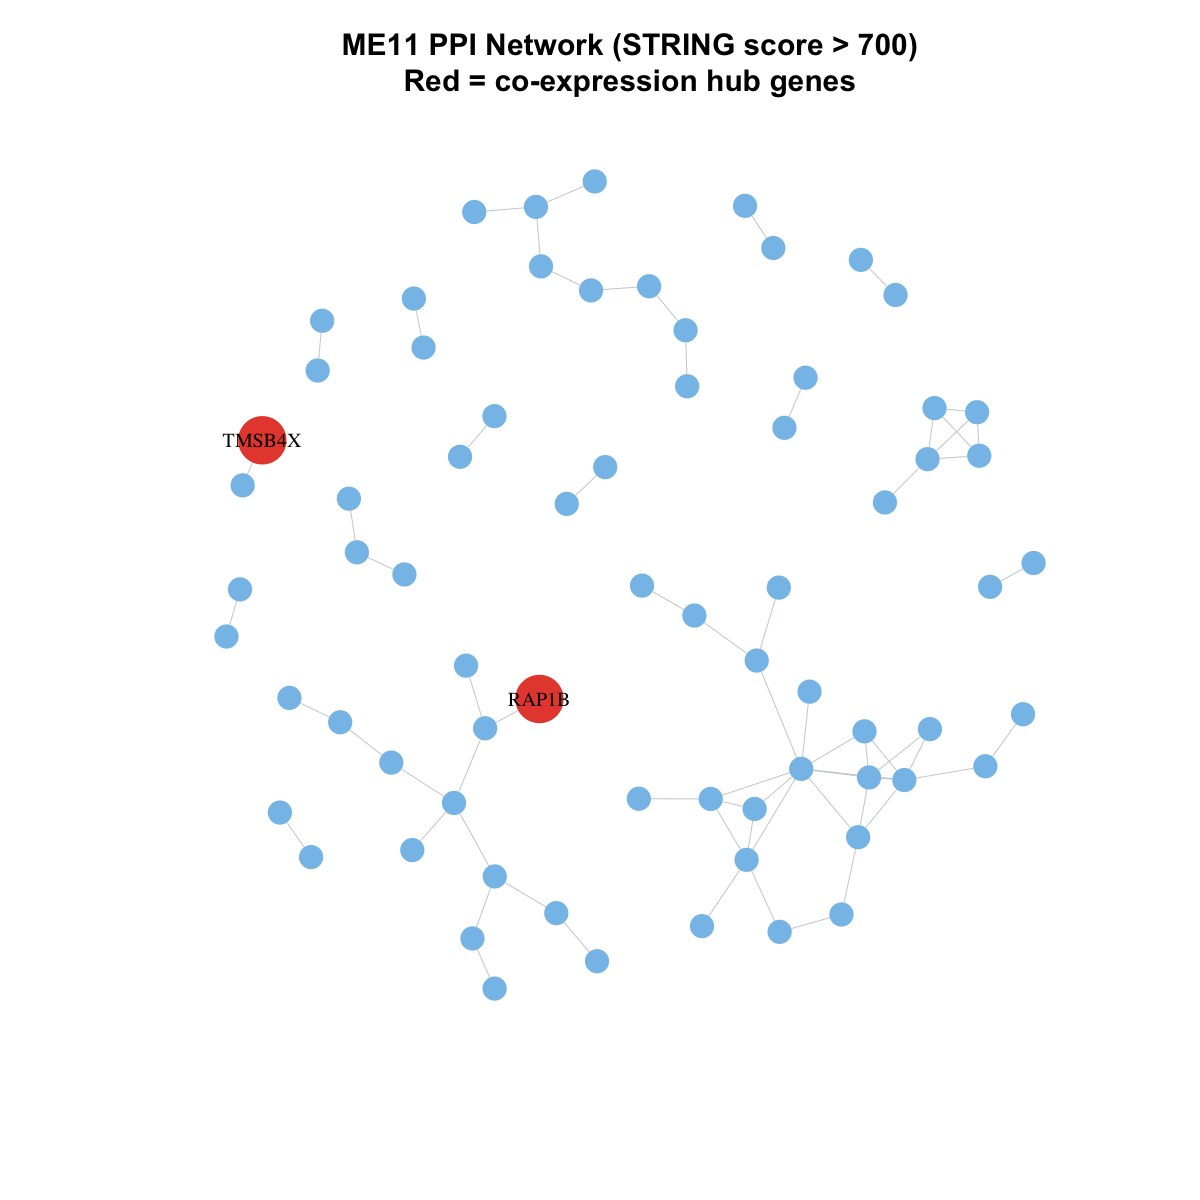
\includegraphics[width=0.9\columnwidth]{ME11_ppi_network.png}
  \caption{ME11 PPI network (STRING score$>700$). Red $=$ co-expression hub genes.
  Hub genes not significantly more central (Wilcoxon $p=0.37$).}
  \label{fig:ppi}
\end{figure}

\subsection{ADHD Validation --- ME11 is ASD-Specific}

No ADHD DE genes at FDR$<0.05$ (n$=76$ underpowered). ME11 module score showed no
significant difference between ADHD and CTRL ($t$-test $p=0.825$; Figure~\ref{fig:adhd}).
Fisher's exact test also non-significant (OR$=0$, $p=1.0$). ME11 is ASD-specific.

\begin{figure}[!htbp]
  \centering
  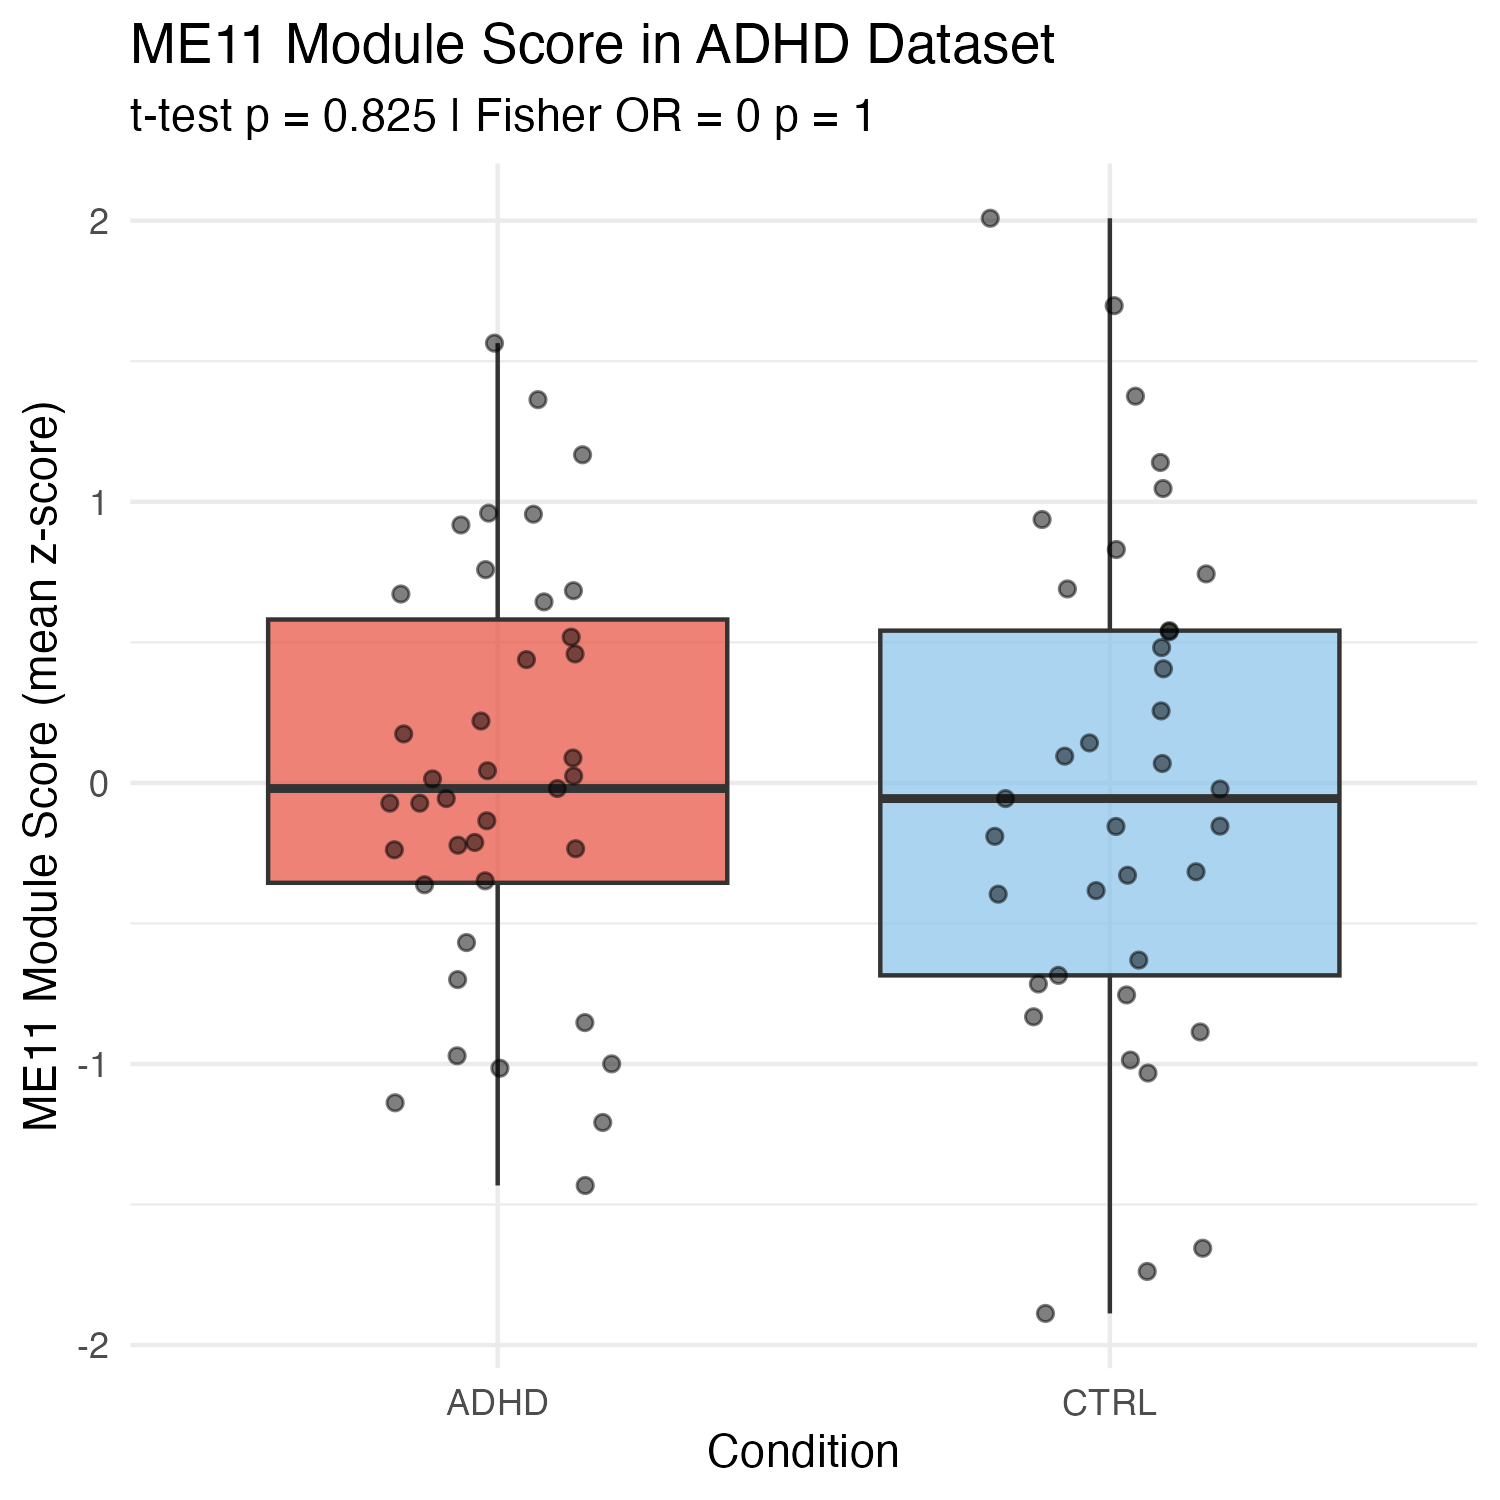
\includegraphics[width=0.85\columnwidth]{ME11_adhd_module_score.png}
  \caption{ME11 module score in ADHD dataset. No significant difference between groups
  ($p=0.825$), establishing ME11 as ASD-specific.}
  \label{fig:adhd}
\end{figure}

\subsection{Reactome Enrichment --- Spliceosomal Module}

Four FDR-significant Reactome pathways identified, all mRNA processing
(Table~\ref{tab:reactome}; Figure~\ref{fig:go}). GO enrichment nominally confirmed:
RNA splicing ($p=8.2\times10^{-5}$), vesicle targeting ($p=2.3\times10^{-4}$),
ribonucleoprotein complex binding ($p=9.0\times10^{-4}$).

\begin{table}[!htbp]
\centering
\caption{FDR-significant Reactome pathways for ME11 genes.}
\label{tab:reactome}
\begin{tabular}{lcc}
\toprule
\rowcolor{teal}\color{white}Pathway & \color{white}Genes & \color{white}FDR \\
\midrule
\rowcolor{lgrey}Pre-mRNA Processing & 12/106 & 0.007 \\
mRNA Splicing --- Major  & 10/106 & 0.007 \\
\rowcolor{lgrey}mRNA Splicing        & 10/106 & 0.007 \\
mRNA Polyadenylation     &  7/106 & 0.033 \\
\bottomrule
\end{tabular}
\end{table}

\begin{figure}[!htbp]
  \centering
  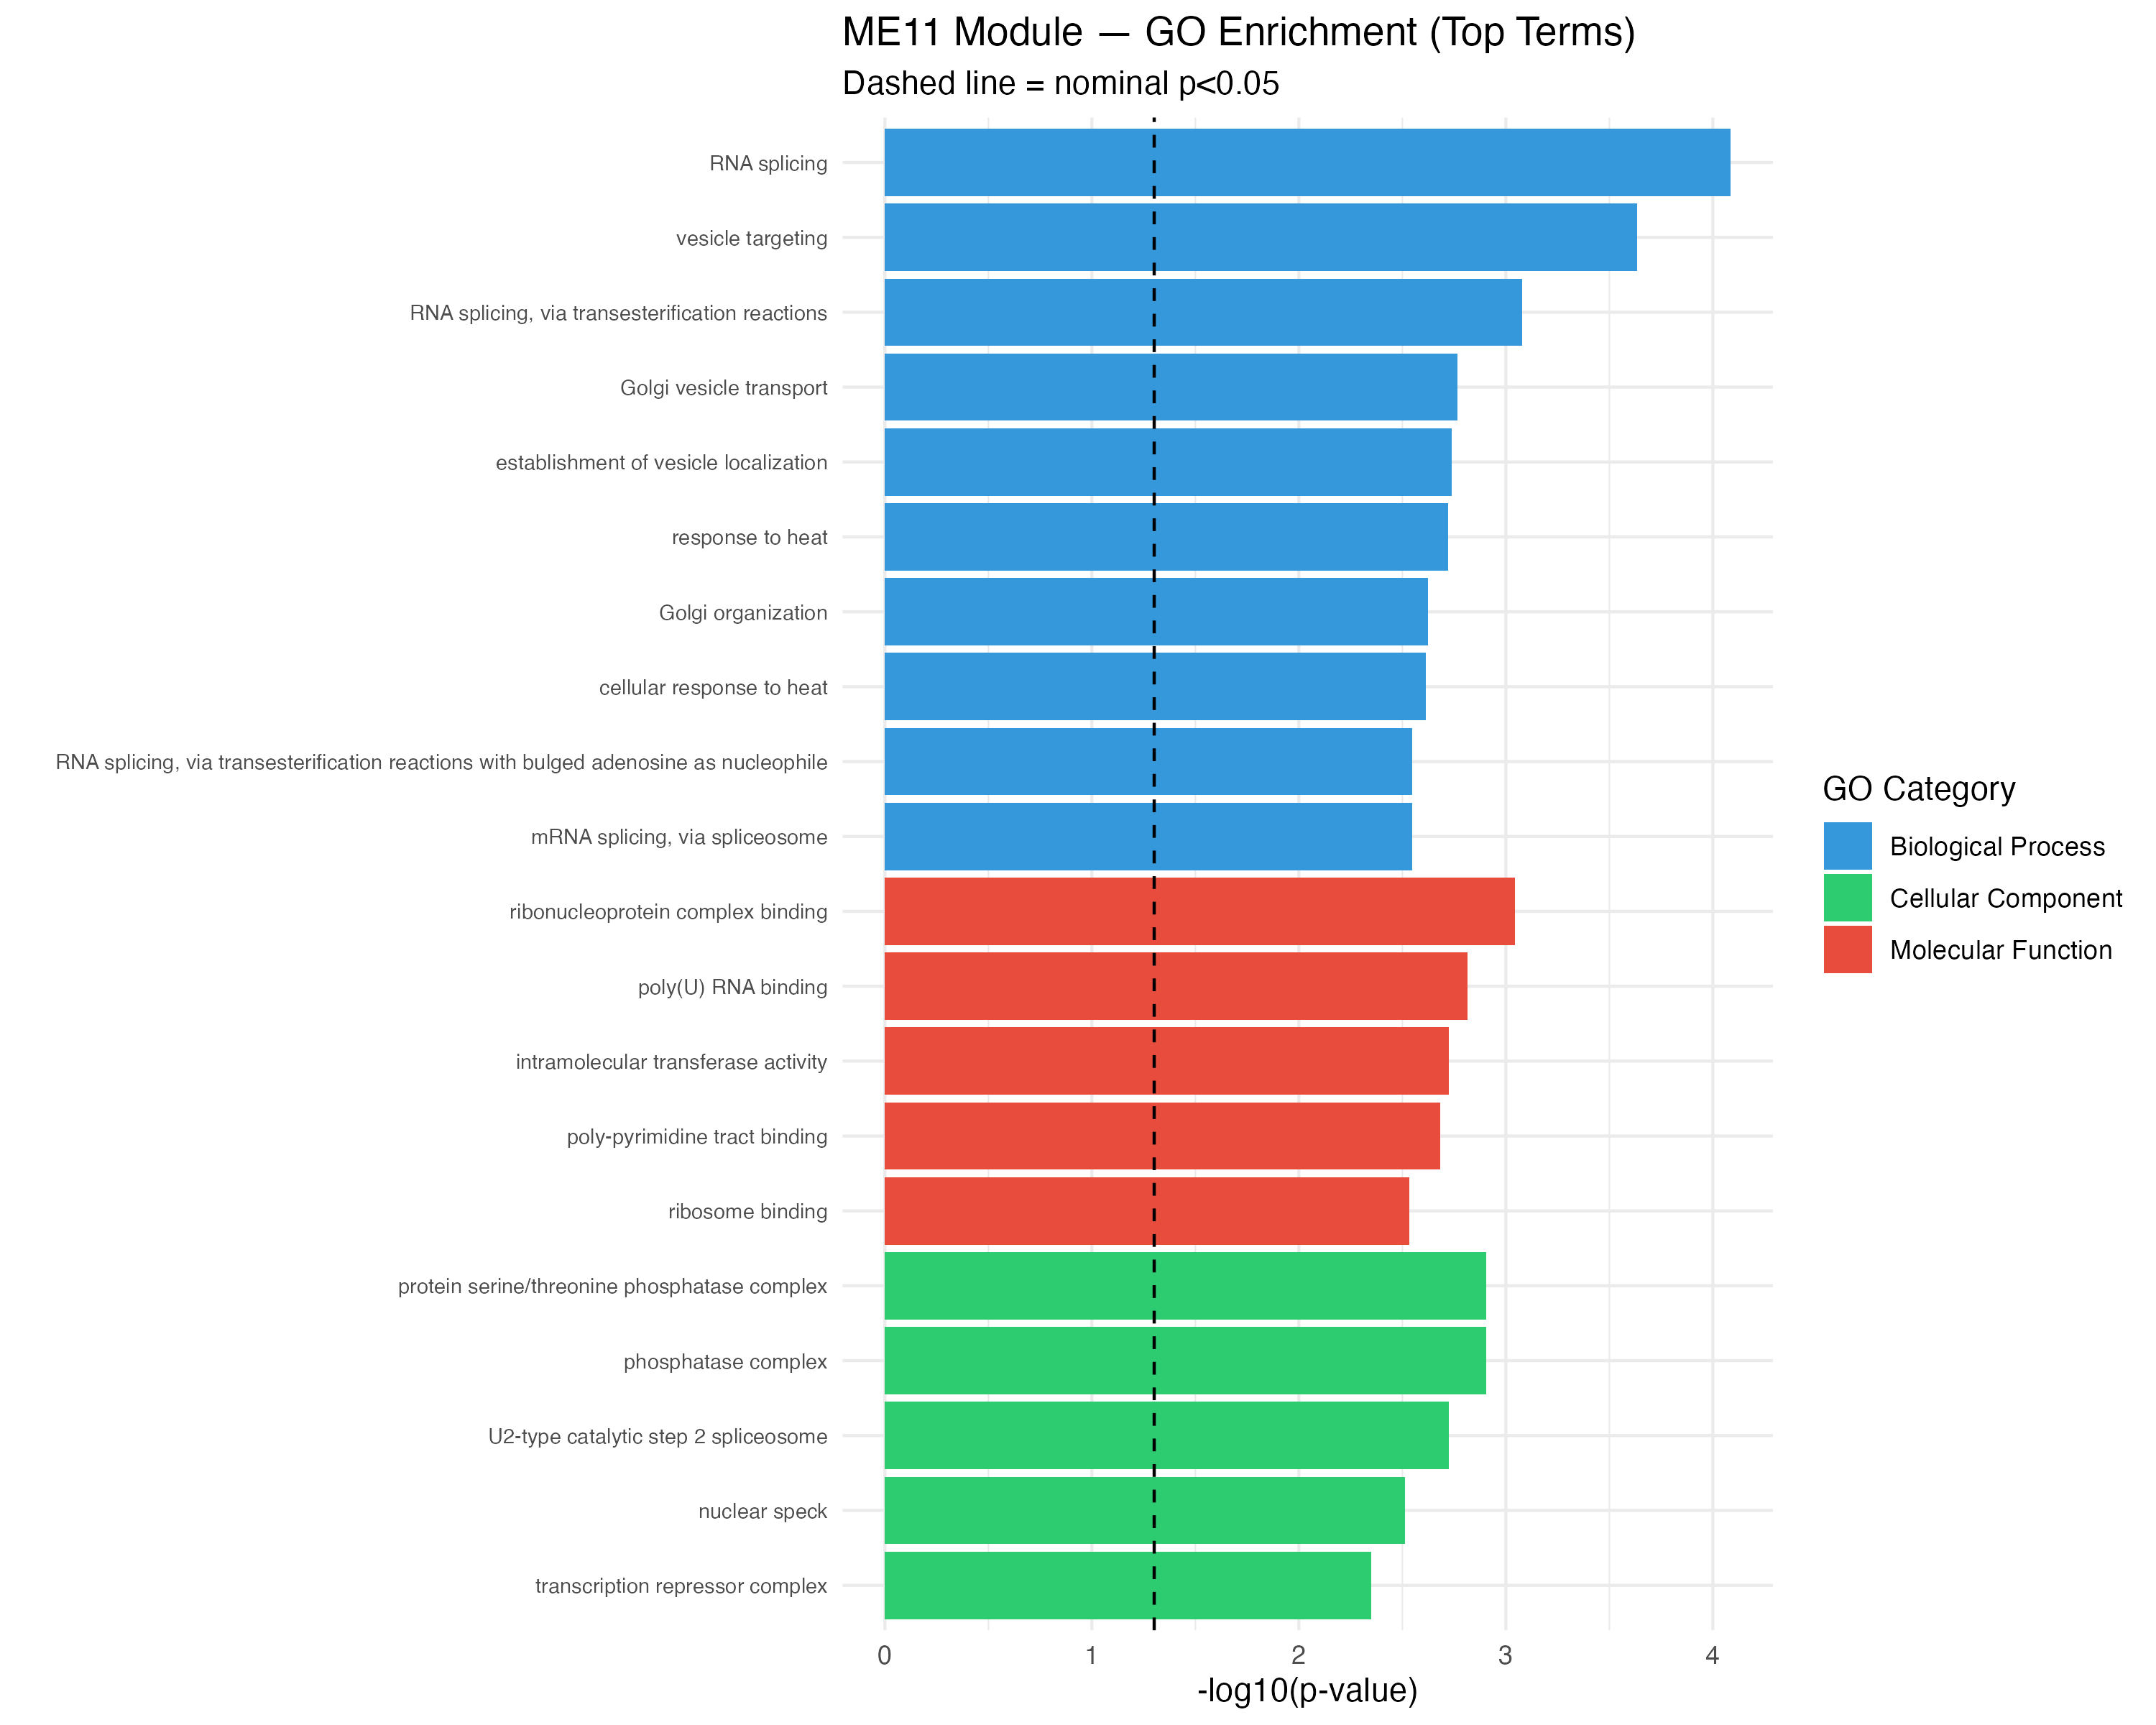
\includegraphics[width=\columnwidth]{ME11_GO_combined.png}
  \caption{GO enrichment for ME11 (top terms, nominal $p<0.05$). RNA splicing is
  the dominant signal ($p=8.2\times10^{-5}$). Dashed line $= p=0.05$ threshold.}
  \label{fig:go}
\end{figure}

% ═══════════════════════════════════════════════════════════════
\section{Discussion}

\subsection{ME11 and Spliceosomal Dysregulation in ASD}

ME11 enrichment for mRNA splicing pathways (FDR$=0.007$) extends the established
ASD spliceosomal dysregulation literature \citep{voineagu2011, parikshak2016,
garcia2025} to peripheral blood transcriptomes. This is the first network-level
evidence that spliceosomal co-expression dysregulation is detectable in ASD blood.
Hub gene biology supports this: ZCCHC10 (zinc finger RNA-binding protein) directly
implicates RNA processing; C1D (nuclear corepressor) links ME11 to transcriptional
silencing, consistent with GO enrichment for transcription repressor complex.

\subsection{PPI Non-Convergence}

Wilcoxon $p=0.37$ indicates ME11 reflects shared upstream transcriptional regulation
rather than a physical protein complex. This is mechanistically informative: the
therapeutic priority should be identifying the upstream transcription factor or
chromatin modifier driving coordinated ME11 repression in ASD, rather than targeting
hub proteins directly.

\subsection{ME11 is ASD-Specific: AuDHD Implications}

ME11's absence of dysregulation in ADHD ($p=0.825$) is consistent with emerging
evidence that ASD and ADHD have dissociable molecular pathways despite shared genetic
liability \citep{mallard2024}. A 2025 Molecular Psychiatry study identified shared
brain connectivity patterns linked to gene expression in children with ASD and/or
ADHD \citep{segura2025}, suggesting shared AuDHD biology exists at the neural
systems level --- but its transcriptomic blood correlate remains to be identified.
ME11 is not the shared component; the WGCNA-PPI framework successfully demonstrates
this distinction. Modules with parallel ASD-ADHD dysregulation remain to be
identified in larger, better-matched datasets.

\subsection{Limitations}

Key limitations: age mismatch between ASD (toddlers, 1--4 years) and ADHD
(adolescents/adults) cohorts; cross-platform differences (microarray vs RNA-seq);
WGCNA not feasible on ADHD (n$=76$, R$^2<0.54$); GO enrichment not FDR-significant
(gene set n$=187$ insufficient for strict correction); no cell-type deconvolution
performed. Future work should prioritize age-matched, brain tissue datasets from
controlled-access repositories (dbGaP, NIMH Data Archive).

% ═══════════════════════════════════════════════════════════════
\section{Conclusion}

ME11 is a robust ASD-associated co-expression module (FDR$=0.0008$) enriched for
spliceosomal pathways (mRNA Splicing FDR$=0.007$) and driven by transcriptional rather
than structural co-regulation (PPI convergence $p=0.37$). ME11 shows no dysregulation
in ADHD ($p=0.825$), establishing it as ASD-specific. The WGCNA-PPI framework
provides a principled, reproducible, openly available approach for distinguishing
disorder-specific from shared molecular networks --- a necessary foundation for
computationally defining AuDHD biology.

% ═══════════════════════════════════════════════════════════════
\section*{Data \& Code Availability}

All analysis code: \url{github.com/vedika13-code/AuDHD-Network}\\
GEO accessions: GSE111175, GSE42133 (ASD); GSE159104 (ADHD).\\
\textit{AI writing assistance (Claude, Anthropic) was used to draft portions of the
manuscript text. All scientific content, analysis, interpretation, and conclusions are
the sole responsibility of the authors.}

% ═══════════════════════════════════════════════════════════════
\section*{References}
\bibliographystyle{plainnat}

% Manual references (replace with .bib file in Overleaf)
\begin{thebibliography}{99}

\bibitem[Vanderbilt(2024)]{vanderbilt2024}
Vanderbilt University Frist Center for Autism and Innovation.
\newblock AuDHD: The Hidden Dynamics of a Dual Diagnosis, 2024.
\newblock \url{https://www.vanderbilt.edu/autismandinnovation/audhd-the-hidden-dynamics-of-a-dual-diagnosis/}

\bibitem[APA(2024)]{apa2024}
American Psychiatric Association.
\newblock When Autism and ADHD Occur Together, 2024.
\newblock \url{https://www.psychiatry.org/news-room/apa-blogs/when-autism-and-adhd-occur-together}

\bibitem[Mallard et~al.(2024)]{mallard2024}
Mallard TT et~al.
\newblock Characterizing genetic pathways unique to autism spectrum disorder at multiple levels
  of biological analysis.
\newblock \textit{medRxiv}, 2024. PMC11481320.

\bibitem[Langfelder and Horvath(2008)]{langfelder2008}
Langfelder P, Horvath S.
\newblock WGCNA: an R package for weighted correlation network analysis.
\newblock \textit{BMC Bioinformatics}, 9:559, 2008.
\newblock \doi{10.1186/1471-2105-9-559}

\bibitem[Voineagu et~al.(2011)]{voineagu2011}
Voineagu I, Wang X, Johnston P, et~al.
\newblock Transcriptomic analysis of autistic brain reveals convergent molecular pathology.
\newblock \textit{Nature}, 474(7351):380--384, 2011.
\newblock \doi{10.1038/nature10110}

\bibitem[Horiuchi et~al.(2021)]{horiuchi2021}
Horiuchi Y et~al.
\newblock Identification of blood transcriptome modules associated with adult autism spectrum disorder.
\newblock \textit{Psychiatry and Clinical Neurosciences}, 2021.

\bibitem[Tomaiuolo et~al.(2023)]{tomaiuolo2023}
Tomaiuolo M et~al.
\newblock Co-expression modules in blood reveal immune dysregulation in ASD discordant siblings.
\newblock \textit{Translational Psychiatry}, 2023.

\bibitem[Thapar et~al.(2022)]{thapar2022}
Thapar A et~al.
\newblock Comprehensive analysis of omics data identifies relevant gene networks for ADHD.
\newblock \textit{Translational Psychiatry}, 12:430, 2022.
\newblock \doi{10.1038/s41398-022-02182-8}

\bibitem[Nangraj et~al.(2020)]{nangraj2020}
Nangraj AS et~al.
\newblock Integrated PPI- and WGCNA-retrieval of hub gene signatures shared between Barrett's
  esophagus and esophageal adenocarcinoma.
\newblock \textit{Frontiers in Pharmacology}, 11:881, 2020.

\bibitem[Davis and Meltzer(2007)]{davis2007}
Davis S, Meltzer PS.
\newblock GEOquery: a bridge between the Gene Expression Omnibus (GEO) and BioConductor.
\newblock \textit{Bioinformatics}, 23(14):1846--1847, 2007.

\bibitem[Johnson et~al.(2007)]{johnson2007}
Johnson WE, Li C, Rabinovic A.
\newblock Adjusting batch effects in microarray expression data using empirical Bayes methods.
\newblock \textit{Biostatistics}, 8(1):118--127, 2007.

\bibitem[Szklarczyk et~al.(2023)]{szklarczyk2023}
Szklarczyk D et~al.
\newblock The STRING database in 2023: protein-protein association networks and functional
  enrichment analyses for any of 12779 organisms.
\newblock \textit{Nucleic Acids Research}, 51(D1):D638--D646, 2023.

\bibitem[Ritchie et~al.(2015)]{ritchie2015}
Ritchie ME et~al.
\newblock limma powers differential expression analyses for RNA-sequencing and microarray studies.
\newblock \textit{Nucleic Acids Research}, 43(7):e47, 2015.

\bibitem[Yu et~al.(2012)]{yu2012}
Yu G, Wang LG, Han Y, He QY.
\newblock clusterProfiler: an R package for comparing biological themes among gene clusters.
\newblock \textit{OMICS}, 16(5):284--287, 2012.

\bibitem[Yu and He(2016)]{yu2016}
Yu G, He QY.
\newblock ReactomePA: an R/Bioconductor package for reactome pathway analysis and visualization.
\newblock \textit{Molecular BioSystems}, 12(2):477--479, 2016.

\bibitem[Parikshak et~al.(2016)]{parikshak2016}
Parikshak NN et~al.
\newblock Genome-wide changes in lncRNA, splicing, and regional gene expression patterns in autism.
\newblock \textit{Nature}, 540(7633):423--427, 2016.

\bibitem[Garcia-Cabau et~al.(2025)]{garcia2025}
Garcia-Cabau C et~al.
\newblock Alternative splicing analysis in a Spanish ASD cohort: in silico prediction and
  characterization.
\newblock \textit{Scientific Reports}, 15:10234, 2025.

\bibitem[Segura et~al.(2025)]{segura2025}
Segura P et~al.
\newblock Connectome-based symptom mapping and in silico related gene expression in children
  with autism and/or attention-deficit/hyperactivity disorder.
\newblock \textit{Molecular Psychiatry}, 2025.
\newblock \doi{10.1038/s41380-025-03205-8}

\end{thebibliography}

\end{document}
